\documentclass[12pt,a4paper]{article}

\usepackage{fontspec}  % Latin Modern by default, supports Ă Â Î Ș Ț
\usepackage[margin=2.5cm]{geometry}
\usepackage{amsmath,amssymb}
\usepackage{graphicx}
\usepackage{booktabs}
\usepackage{array}
\usepackage{float}
\usepackage{caption}
\usepackage{xcolor}
\usepackage{listings}
\usepackage[colorlinks=true,linkcolor=blue,urlcolor=blue,citecolor=blue]{hyperref}

\captionsetup{labelsep=colon}
\renewcommand{\lstlistingname}{Listing}

\definecolor{codebg}{gray}{0.96}
\definecolor{codeframe}{gray}{0.85}
\definecolor{codecomment}{rgb}{0.0,0.55,0.0}
\definecolor{codenumber}{gray}{0.5}

\lstset{
  language=Python,
  basicstyle=\ttfamily\footnotesize,
  keywordstyle=\color{blue},
  commentstyle=\color{codecomment},
  stringstyle=\color{black},
  numbers=left,
  numberstyle=\tiny\color{codenumber},
  numbersep=6pt,
  backgroundcolor=\color{codebg},
  frame=single,
  rulecolor=\color{codeframe},
  framerule=0.4pt,
  showstringspaces=false,
  breaklines=true,
  tabsize=4,
  columns=fullflexible,
  keepspaces=true,
  captionpos=b,
  xleftmargin=1.5em,
  framexleftmargin=1.5em
}

\begin{document}

% ------------------------------------------------------------------ title page
\begin{titlepage}
  \centering
  \vspace*{0.5cm}
  {\bfseries Ministerul Educaţiei şi Cercetării al Republicii Moldova\par}
  \vspace{0.25cm}
  {\bfseries Universitatea Tehnică a Moldovei\par}
  \vspace{0.25cm}
  {\bfseries Facultatea Calculatoare, Informatică şi Microelectronică\par}

  \vspace{4cm}
  {\LARGE Laboratory work 1:\par}
  \vspace{0.3cm}
  {\Large\bfseries The Caesar Cipher\par}
  \vspace{0.2cm}
  {\large\bfseries (Classic and with a Keyword Permutation)\par}

  \vspace{3cm}
  \hspace{4cm}
  \begin{minipage}{0.5\textwidth}
    \textbf{Elaborated:}\\
    st. gr. FAF-243 Morari Veaceslav

    \vspace{0.5cm}
    \textbf{Verified:}\\
    asist. univ. Zaica Maia
  \end{minipage}

  \vfill
  {\large Chişinău -- 2026\par}
\end{titlepage}

% ------------------------------------------------------------------ contents
\tableofcontents
\newpage

% ------------------------------------------------------------------ 1
\section{ALGORITHM ANALYSIS}

\subsection{Objective}

Study the Caesar cipher, understand why its small key space makes it insecure,
strengthen it with a keyword-based permutation of the alphabet, and implement both
versions for the Romanian alphabet.

\subsection{Tasks}

The tasks of this laboratory work are the following. First, implement the Caesar cipher
for the Romanian alphabet ($n = 31$) using only the letter encoding from the assignment
(A $=0$, Ă $=1$, \ldots, Z $=30$), with a key from 1 to 30 (Task 1.1). Second, implement
the Caesar cipher with two keys: a numeric shift and a keyword of at least 7 letters that
permutes the alphabet (Task 1.2). In both tasks the text is converted to uppercase, spaces
are removed, and any invalid key or character must produce a clear error message and a
new request for the value. Finally, draw conclusions about the security of the two ciphers.

\subsection{Theoretical Notes}

The \textbf{Caesar cipher} is a substitution cipher: every letter of the plaintext is
replaced by the letter found a fixed number of positions $k$ further along the alphabet.
The key $k$ is the same for encryption and decryption, $k \in \{1, 2, \ldots, n-1\}$,
where $n$ is the length of the alphabet. If $x$ and $y$ are the numeric codes of a
plaintext and of a ciphertext letter, then
\begin{align*}
  c &= e_k(x) = (x + k) \bmod n, \\
  m &= d_k(y) = (y - k) \bmod n.
\end{align*}
When $y - k$ is negative, $n$ is added to bring the result back into the range
$0 \ldots n-1$. For the Romanian alphabet, for example, with $k = 3$:
$e_3(\text{Ș}) = (22 + 3) \bmod 31 = 25 = \text{U}$ and
$d_3(\text{A}) = (0 - 3) \bmod 31 = 28 = \text{X}$.

The cipher has only $n - 1$ useful keys: 25 for English and 30 for Romanian. An attacker
can try all of them in a fraction of a second (\textit{brute-force attack}) and keep the
only result that reads as meaningful text.

The \textbf{Caesar cipher with a permutation} uses a second key, a \textit{keyword} $k_2$,
to reorder the alphabet. The keyword letters are written first, each only at its first
occurrence, followed by the remaining letters in their natural order. The shift $k_1$ is then
applied over the permuted alphabet $\pi$, where $\mathrm{pos}(\cdot)$ is the position of a
letter in $\pi$:
\begin{align*}
  c &= \pi\left[(\mathrm{pos}(x) + k_1) \bmod n\right], \\
  m &= \pi\left[(\mathrm{pos}(y) - k_1) \bmod n\right].
\end{align*}
The number of key pairs $(k_1, k_2)$ is $n! \cdot (n-1)$. For Romanian this gives
$31! \cdot 30 \approx 2.47 \cdot 10^{35}$, so exhaustive search is no longer practical.
However, the cipher remains \textit{monoalphabetic}: the same plaintext letter is always
replaced by the same ciphertext letter, so it can still be broken by
\textit{frequency analysis}.

% ------------------------------------------------------------------ 2
\section{Introduction}

The Caesar cipher is one of the oldest known encryption methods. It is named after Julius
Caesar, who is said to have used it with the key $k = 3$ to communicate with his generals.
Today it has no practical security value, but it is the standard starting point for
studying classical cryptography: it shows the idea of a secret key, modular arithmetic over
an alphabet, and the difference between a large key space and real security.

Both versions in this work operate on the 31 letters of the Romanian alphabet, which
includes the five diacritic letters Ă, Â, Î, Ș and Ț.

\subsection{Alphabet Encoding}

The letters are encoded only with the table from the assignment (Table~\ref{tab:alphabet}).
Built-in character encodings (ASCII or Unicode code points) are not used to compute the
shift.

\begin{table}[H]
  \centering
  \caption{Letter encoding of the Romanian alphabet ($n = 31$).}
  \label{tab:alphabet}
  \setlength{\tabcolsep}{2.1pt}
  \scriptsize
  \begin{tabular}{l*{31}{c}}
    \toprule
    \textbf{Letter} & A & Ă & Â & B & C & D & E & F & G & H & I & Î & J & K & L & M & N & O & P & Q & R & S & Ș & T & Ț & U & V & W & X & Y & Z \\
    \textbf{Code}   & 0 & 1 & 2 & 3 & 4 & 5 & 6 & 7 & 8 & 9 & 10 & 11 & 12 & 13 & 14 & 15 & 16 & 17 & 18 & 19 & 20 & 21 & 22 & 23 & 24 & 25 & 26 & 27 & 28 & 29 & 30 \\
    \bottomrule
  \end{tabular}
\end{table}

\subsection{Input Format}

The key (and the shift $k_1$ in Task 1.2) must be an integer from 1 to 30 inclusive. The
text may contain only Romanian letters, in upper or lower case, and spaces; spaces are
removed and the text is converted to uppercase before encryption. The keyword must contain
only Romanian letters and have at least 7 letters. The letters Ș and Ț are also accepted
when typed with a cedilla (Ş, Ţ), so text typed on different keyboards is handled the same
way.

% ------------------------------------------------------------------ 3
\section{IMPLEMENTATION}

Both tasks are implemented in Python 3 in a single console program,
\texttt{caesar\_cipher.py}. A menu lets the user choose Task 1.1 or Task 1.2, then the
operation (encryption or decryption), the key(s) and the text. A separate file,
\texttt{test\_caesar\_cipher.py}, contains unit tests for the main functions.

\subsection{Letter Encoding}

\begin{lstlisting}[caption={Romanian alphabet and letter normalization}]
ALPHABET = ["A", "Ă", "Â", "B", "C", "D", "E", "F", "G", "H", "I", "Î", "J",
            "K", "L", "M", "N", "O", "P", "Q", "R", "S", "Ș", "T", "Ț", "U",
            "V", "W", "X", "Y", "Z"]
LOWERCASE = ["a", "ă", "â", "b", "c", "d", "e", "f", "g", "h", "i", "î", "j",
             "k", "l", "m", "n", "o", "p", "q", "r", "s", "ș", "t", "ț", "u",
             "v", "w", "x", "y", "z"]
N = len(ALPHABET)  # 31

TO_UPPER = {}
for upper, lower in zip(ALPHABET, LOWERCASE):
    TO_UPPER[upper] = upper
    TO_UPPER[lower] = upper
TO_UPPER.update({"Ş": "Ș", "ş": "Ș", "Ţ": "Ț", "ţ": "Ț"})
\end{lstlisting}

The alphabet is stored as a list in the exact order of Table~\ref{tab:alphabet}, so the
code of a letter is simply its index. The dictionary \texttt{TO\_UPPER} maps every accepted
character to its uppercase letter, including the cedilla variants of Ș and Ț.

\subsection{Input Validation}

\begin{lstlisting}[caption={Text normalization and key validation}]
def normalize_text(text):
    text = unicodedata.normalize("NFC", text)
    result = []
    for ch in text:
        if ch == " ":
            continue
        if ch not in TO_UPPER:
            return None, ch          # first rejected character
        result.append(TO_UPPER[ch])
    return "".join(result), None

def parse_key(raw):
    raw = raw.strip()
    if not raw.isdigit():
        return None
    key = int(raw)
    return key if MIN_KEY <= key <= MAX_KEY else None
\end{lstlisting}

\texttt{normalize\_text} removes spaces, converts the text to uppercase and returns the
first character that is not a Romanian letter, so the error message can name it.
\texttt{parse\_key} accepts only an integer from 1 to 30; inputs such as \texttt{0},
\texttt{35}, \texttt{-1}, \texttt{2.5} or \texttt{abc} are rejected. The functions
\texttt{ask\_key}, \texttt{ask\_text} and \texttt{ask\_keyword} repeat the question until a
valid value is entered; \texttt{ask\_keyword} also checks the minimum length of 7 letters.

\subsection{Task 1.1: The Caesar Cipher}

\subsubsection{Algorithm Description}

Each letter of the prepared text is replaced by its code $x$, the code is shifted by the key
modulo 31, and the letter with the new code is written to the ciphertext. Decryption is the
same operation with the key $-k$. Python's \texttt{\%} operator always returns a value from
0 to $n-1$, so $(y - k) \bmod n$ never becomes negative and no extra correction is needed.

\subsubsection{Implementation}

\begin{lstlisting}[caption={Shift over an alphabet and the classic Caesar cipher}]
def shift_text(text, key, alphabet):
    position = {letter: i for i, letter in enumerate(alphabet)}
    return "".join(alphabet[(position[ch] + key) % N] for ch in text)

def caesar_encrypt(text, k):
    return shift_text(text, k, ALPHABET)          # c = (x + k) mod n

def caesar_decrypt(text, k):
    return shift_text(text, -k, ALPHABET)         # m = (y - k) mod n
\end{lstlisting}

One function, \texttt{shift\_text}, does the work for both tasks: Task 1.1 passes the normal
alphabet, Task 1.2 passes the permuted one.

\subsubsection{Results}

Figure~\ref{fig:t11} shows the encryption of the message ``Criptografie și securitate''
with $k = 3$ and the decryption of the obtained ciphertext. Table~\ref{tab:check11} checks the
first letters by hand.

\begin{figure}[H]
  \centering
  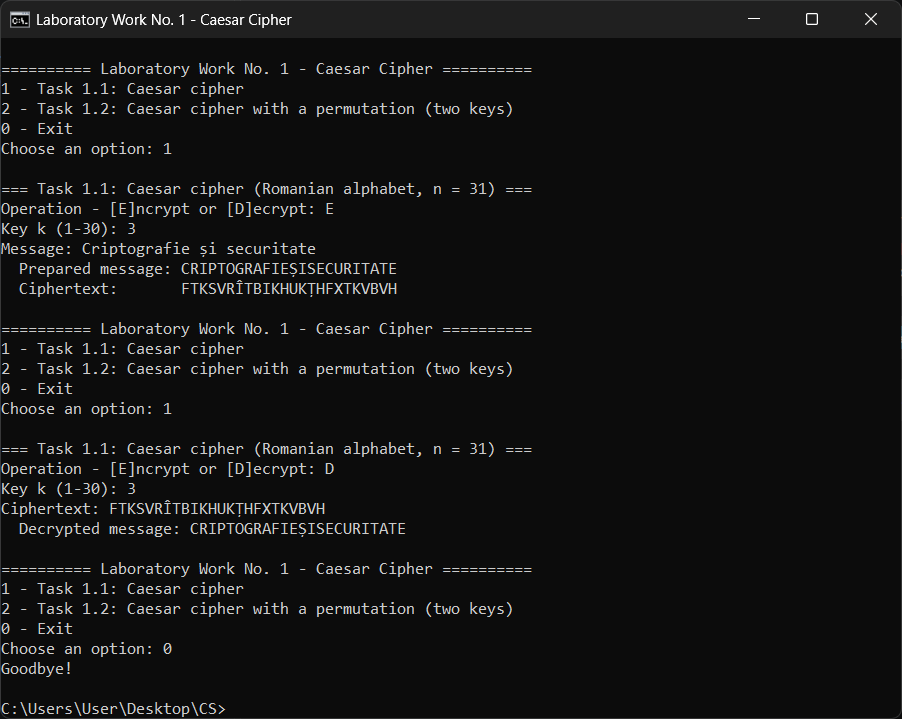
\includegraphics[width=0.8\textwidth]{../screenshots/fig1_task1_1_encrypt_decrypt.png}
  \caption{Task 1.1: encryption and decryption with $k = 3$.}
  \label{fig:t11}
\end{figure}

\begin{table}[H]
  \centering
  \caption{Manual check of Task 1.1 ($k = 3$).}
  \label{tab:check11}
  \begin{tabular}{cccc}
    \toprule
    \textbf{Letter $m$} & $x$ & $(x + 3) \bmod 31$ & \textbf{Letter $c$} \\
    \midrule
    C & 4  & 7  & F \\
    R & 20 & 23 & T \\
    I & 10 & 13 & K \\
    P & 18 & 21 & S \\
    Ș & 22 & 25 & U \\
    \bottomrule
  \end{tabular}
\end{table}

\subsection{Task 1.2: The Caesar Cipher with a Permutation}

\subsubsection{Algorithm Description}

The keyword is normalized like the text and must have at least 7 letters. The permuted
alphabet is built by going through the keyword and then through the whole alphabet, adding
each letter only the first time it appears; the result always contains all 31 letters
exactly once. The program prints the permuted alphabet under the original one, so the result
can be checked by hand. Encryption and decryption use the same \texttt{shift\_text} function,
but over the permuted alphabet.

\subsubsection{Implementation}

\begin{lstlisting}[caption={Permuted alphabet and the Caesar cipher with two keys}]
def build_permuted_alphabet(keyword):
    permuted = []
    for letter in keyword + "".join(ALPHABET):
        if letter not in permuted:
            permuted.append(letter)
    return permuted

def caesar2_encrypt(text, k1, keyword):
    return shift_text(text, k1, build_permuted_alphabet(keyword))

def caesar2_decrypt(text, k1, keyword):
    return shift_text(text, -k1, build_permuted_alphabet(keyword))
\end{lstlisting}

\subsubsection{Results}

For $k_1 = 5$ and $k_2 = $ CRIPTOGRAFIE the keyword contributes 10 distinct letters (the
second R and the second I are dropped). Table~\ref{tab:perm} shows the resulting permuted
alphabet and the substitution it produces.

\begin{table}[H]
  \centering
  \caption{Caesar cipher with keys $k_1 = 5$ and $k_2 = $ CRIPTOGRAFIE.}
  \label{tab:perm}
  \setlength{\tabcolsep}{2.1pt}
  \scriptsize
  \begin{tabular}{l*{31}{c}}
    \toprule
    $x$        & 0 & 1 & 2 & 3 & 4 & 5 & 6 & 7 & 8 & 9 & 10 & 11 & 12 & 13 & 14 & 15 & 16 & 17 & 18 & 19 & 20 & 21 & 22 & 23 & 24 & 25 & 26 & 27 & 28 & 29 & 30 \\
    $m$        & C & R & I & P & T & O & G & A & F & E & Ă & Â & B & D & H & Î & J & K & L & M & N & Q & S & Ș & Ț & U & V & W & X & Y & Z \\
    \midrule
    $x+k_1$    & 5 & 6 & 7 & 8 & 9 & 10 & 11 & 12 & 13 & 14 & 15 & 16 & 17 & 18 & 19 & 20 & 21 & 22 & 23 & 24 & 25 & 26 & 27 & 28 & 29 & 30 & 0 & 1 & 2 & 3 & 4 \\
    $c$        & O & G & A & F & E & Ă & Â & B & D & H & Î & J & K & L & M & N & Q & S & Ș & Ț & U & V & W & X & Y & Z & C & R & I & P & T \\
    \bottomrule
  \end{tabular}
\end{table}

Figure~\ref{fig:t12} shows the encryption of ``Țara mea Moldova'' and the decryption of the
ciphertext \texttt{YBGBȚHBȚĂȘLĂCB}. For example, Ț has position 24, so it becomes the letter
at position $(24 + 5) \bmod 31 = 29$, which is Y; A (position 7) becomes B (position 12).

\begin{figure}[H]
  \centering
  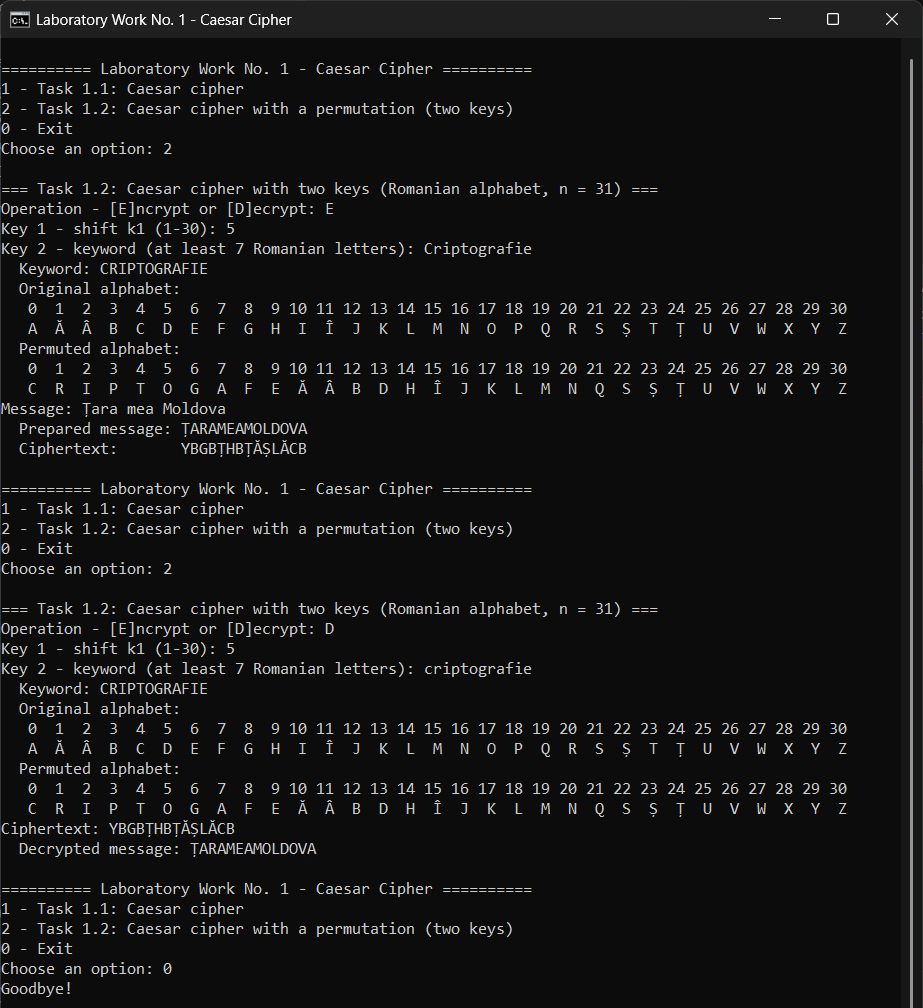
\includegraphics[height=0.62\textheight]{../screenshots/fig3_task1_2_encrypt_decrypt.png}
  \caption{Task 1.2: permuted alphabet, encryption and decryption.}
  \label{fig:t12}
\end{figure}

\subsection{Handling of Invalid Input}

Figures~\ref{fig:inv11} and~\ref{fig:inv12} show the messages displayed for invalid input:
a key outside the range 1--30, a key that is not a number, a message with digits or
punctuation, a keyword that is too short and a keyword with an invalid character. In every
case the program states the allowed values and asks for the value again.

\begin{figure}[H]
  \centering
  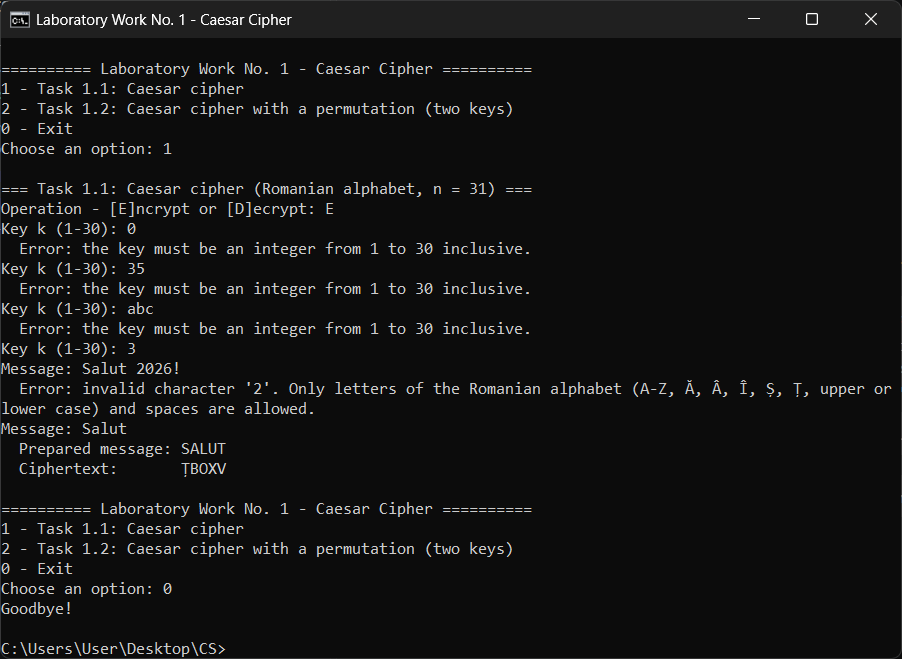
\includegraphics[width=0.8\textwidth]{../screenshots/fig2_task1_1_invalid_input.png}
  \caption{Task 1.1: messages for a wrong key and an invalid character.}
  \label{fig:inv11}
\end{figure}

\begin{figure}[H]
  \centering
  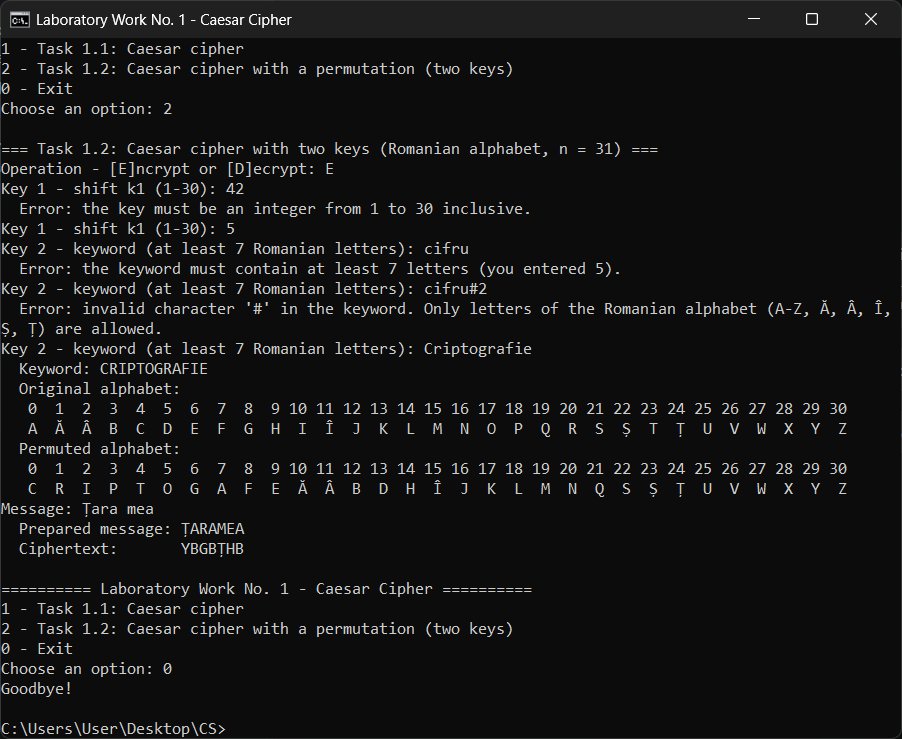
\includegraphics[width=0.8\textwidth]{../screenshots/fig4_task1_2_invalid_input.png}
  \caption{Task 1.2: messages for a wrong shift, a short keyword and an invalid character.}
  \label{fig:inv12}
\end{figure}

\subsection{Comparison: Classic vs.\ Permutation}

The unit tests check text normalization, key validation, the wrap-around
(Z $+ 1 =$ A), the permuted alphabet, and that decryption restores the message for all 30
keys in both versions; all 6 tests pass. Table~\ref{tab:compare} compares the two versions.

\begin{table}[H]
  \centering
  \caption{Comparison of the two versions of the Caesar cipher ($n = 31$).}
  \label{tab:compare}
  \begin{tabular}{lcc}
    \toprule
                         & \textbf{Classic} & \textbf{With permutation} \\
    \midrule
    Keys                 & $k \in \{1, \ldots, 30\}$ & $k_1 \in \{1, \ldots, 30\}$, keyword $k_2$ \\
    Number of keys       & 30 & $31! \cdot 30 \approx 2.47 \cdot 10^{35}$ \\
    Brute-force attack   & trivial & impractical \\
    Frequency analysis   & vulnerable & vulnerable \\
    \bottomrule
  \end{tabular}
\end{table}

% ------------------------------------------------------------------ 4
\section{CONCLUSION}

Within this laboratory work, the Caesar cipher and the Caesar cipher with a keyword
permutation were implemented in Python for the 31-letter Romanian alphabet. Both versions
encrypt and decrypt correctly, which was confirmed by unit tests for all 30 keys and by
manual checks of the substitution tables.

\textbf{The classic Caesar cipher is not secure.} Over the Romanian alphabet it has only 30
keys, so an attacker can try every key and keep the only result that reads as Romanian text.
Such an attack takes less than a second even by hand-written code.

\textbf{The keyword permutation removes the brute-force problem, but not the main
weakness.} The key space grows to $31! \cdot 30 \approx 2.47 \cdot 10^{35}$ pairs, which
cannot be searched exhaustively. However, the cipher is still a monoalphabetic substitution:
each plaintext letter is always replaced by the same ciphertext letter, so letter
frequencies of the language (in Romanian, E, A and I are the most common) remain visible in
the ciphertext. With a long enough message, frequency analysis recovers the text without
knowing the key. A large key space is therefore necessary, but not sufficient for security.

In conclusion, during this work I learned how to encode a non-English alphabet with my own
table instead of ASCII or Unicode codes, how to handle modular arithmetic correctly when
$y - k$ is negative, how to build a permuted alphabet from a keyword without repeating
letters, and how to validate user input with clear error messages.

\section{SOURCE CODE}

The full source code is available on GitHub:
\url{https://github.com/veacheslavv/CS_Labs/tree/main/Lab1}

\end{document}
